\documentclass[12pt]{article}
\input{bayesuvius.sty}
\begin{document}

\begin{figure}[h!]\centering
\begin{minipage}{.5\linewidth}
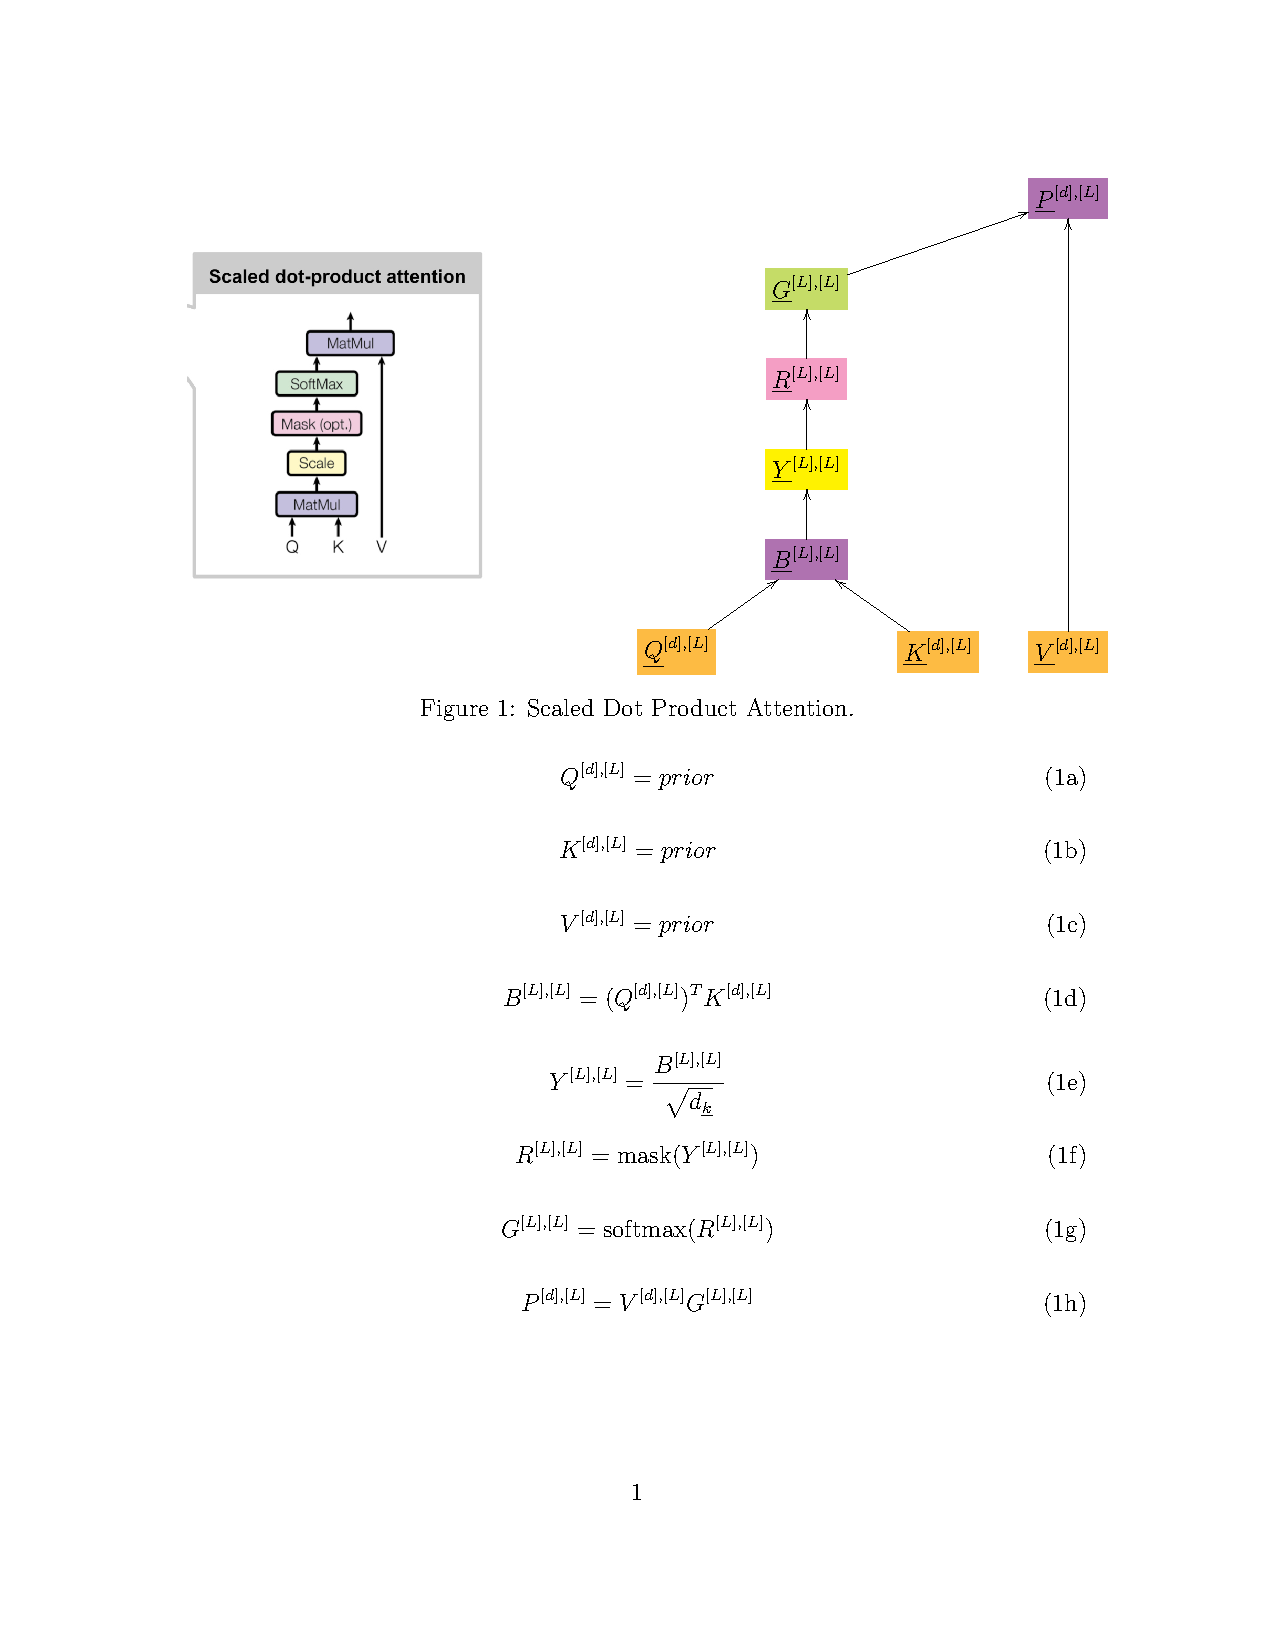
\includegraphics[width=2in]{scaled-dot-prod-att.jpg}
\end{minipage}%blank lines between minispaces breaks this
\begin{minipage}{.5\linewidth}
$$\xymatrix{
&&&*+[F*:Orchid]{\underline{A}^{[d], [\ell]}}
\\
&*+[F*:SpringGreen]{\underline{G}^{[\ell], [\ell]}}\ar[urr]&&
\\
&*+[F*:Lavender]{\underline{R}^{[\ell], [\ell]}}\ar[u]&&
\\
&*+[F*:yellow]{\underline{Y}^{[\ell],[\ell]}}\ar[u]&&
\\
&*+[F*:Dandelion]{\underline{B}^{[\ell], [\ell]}}\ar[u]&&
\\
*+[F*:Orchid]{\underline{Q}^{[d],[\ell]}}\ar[ur]&&*+[F*:Orchid]{\underline{K}^{[d],[\ell]}}\ar[ul]&*+[F*:Orchid]{\underline{V}^{[d],[\ell]}}\ar[uuuuu]
}$$
\end{minipage}
\caption{Scaled Dot Product Attention.}
\label{fig-texnn-for-scaled-dot-prod-att}
\end{figure}

\begin{subequations}

\begin{equation}\color{blue}
A^{[d], [\ell]} = V^{[d],[\ell]} G^{[\ell], [\ell]}
\label{eq-A-fun-scaled-dot-prod-att}
\end{equation}

\begin{equation}\color{blue}
B^{[\ell], [\ell]} = (Q^{[d],[\ell]})^T K^{[d],[\ell]}
\label{eq-B-fun-scaled-dot-prod-att}
\end{equation}

\begin{equation}\color{blue}
G^{[\ell], [\ell]} = {\rm softmax}(R^{[\ell], [\ell]})
\label{eq-G-fun-scaled-dot-prod-att}
\end{equation}

\begin{equation}\color{blue}
K^{[d],[\ell]} = prior
\label{eq-K-fun-scaled-dot-prod-att}
\end{equation}

\begin{equation}\color{blue}
Q^{[d],[\ell]} = prior
\label{eq-Q-fun-scaled-dot-prod-att}
\end{equation}

\begin{equation}\color{blue}
R^{[\ell], [\ell]} = {\rm mask}(Y^{[\ell],[\ell]})
\label{eq-R-fun-scaled-dot-prod-att}
\end{equation}

\begin{equation}\color{blue}
V^{[d],[\ell]} = prior
\label{eq-V-fun-scaled-dot-prod-att}
\end{equation}

\begin{equation}\color{blue}
Y^{[\ell],[\ell]} = \frac{B^{[\ell], [\ell]}}{\sqrt{d_\rvk}}
\label{eq-Y-fun-scaled-dot-prod-att}
\end{equation}

\end{subequations}


\end{document}  
